\documentclass{article}
\usepackage{graphicx}
\title{Investing notes}
\date{10-19-2022}
\author{Tommy Bui}

\begin{document}
	\maketitle
	\newpage
	\pagenumbering{arabic}

	\section{Analyzing a stock from Yahoo Finance} 
	
	\begin{figure}[h!]
		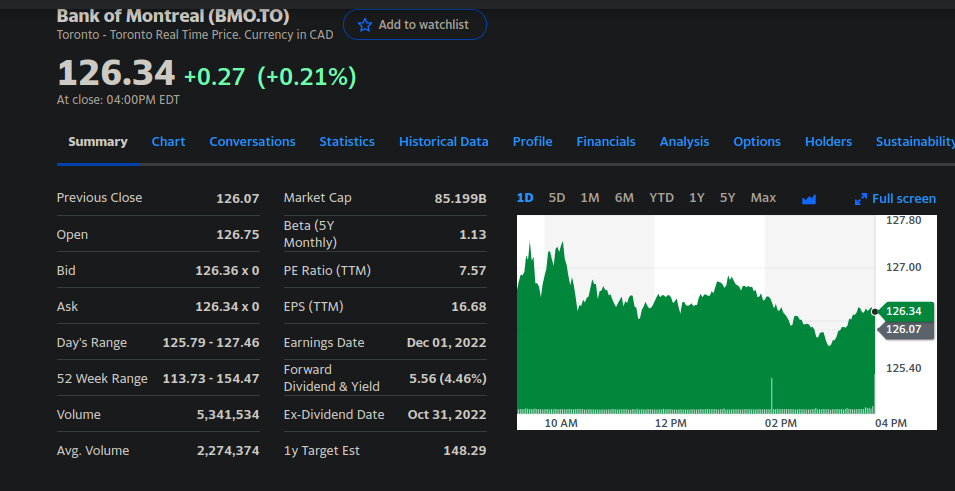
\includegraphics[width=\linewidth]{InvestingPics/figure1.png}
		\caption{View of \$BMO.TO in Yahoo Finance}
		\label{fig:chart1}
	\end{figure}

	%Figure \ref{fig:chart1} is a chart of BMO.TO

	\subsection{Analyzing the Summary Tab}

	\begin{itemize}
		\item {\bf Previous Close:} represents the last closing price reported of a security during a given time period; A security's previous close is an important value that is used by investors to chart gap patterns which can show substantial changes from a previous close to a new open.
	\end{itemize}

\end{document}
